\documentclass[conference]{IEEEtran}
\usepackage{cite}
\usepackage{graphicx}
\usepackage{multirow}
\usepackage{amssymb}
\usepackage{siunitx}
\usepackage{dcolumn}
\usepackage{color, colortbl}
\usepackage{balance}
%\usepackage{url}
\usepackage{subcaption}
\definecolor{Gray}{gray}{0.9}

\usepackage[hidelinks]{hyperref}


\usepackage{fontenc}

\clubpenalty = 10000
\widowpenalty = 10000
\displaywidowpenalty = 10000

% correct bad hyphenation here
\hyphenation{op-tical net-works semi-conduc-tor}


\IEEEoverridecommandlockouts

\begin{document}


%
% paper title
% Titles are generally capitalized except for words such as a, an, and, as,
% at, but, by, for, in, nor, of, on, or, the, to and up, which are usually
% not capitalized unless they are the first or last word of the title.
% Linebreaks \\ can be used within to get better formatting as desired.
% Do not put math or special symbols in the title.
\title{Flower: Navigating Program Flow in the IDE}


% author names and affiliations
% use a multiple column layout for up to three different
% affiliations

\author{\IEEEauthorblockN{Justin Smith, Chris Brown, and Emerson Murphy-Hill}
\IEEEauthorblockA{Department of Computer Science\\
North Carolina State University\\
Raleigh, North Carolina\\
Email: jssmit11@ncsu.edu, dcbrow10@ncsu.edu, emerson@csc.ncsu.edu}
}

%978-1-5386-0443-4/17/$31.00 ©2017 IEEE
\IEEEpubid{\makebox[\columnwidth]{978-1-5386-0443-4/17/\$31.00 \copyright 2017 IEEE \hfill} \hspace{\columnsep}\makebox[\columnwidth]{ }}

\maketitle

% As a general rule, do not put math, special symbols or citations
% in the abstract
\begin{abstract}
Program navigation is a critical task for software developers. 
%Many tools and approaches have been proposed to aide developers in navigating programs.
%In this work we present a tool, Flower, that enables developers 
State-of-the-art tools have been shown to support effective program navigation strategies, and do so by adding widgets, secondary views, and visualizations to the screen. 
In this work, we build on prior work by exploring what types of navigation can be supported with relatively few interface elements.
To that end, we designed and implemented a prototype tool, named Flower, that supports structural program navigation while maintaining a minimalistic interface.
Flower enables developers to simultaneously navigate control flow and data flow within the Eclipse Integrated Development Environment.
Based on a preliminary evaluation with eight programmers, Flower succeeds when call graphs contained relatively few branches, but was strained by complex program structures.
%We present a different way to do things... enable the navigation control flow and data flow simultaneously using minimal interface alterations.
%Something about tradeoffs.
%For simple sub-tasks tool was effective with very few interface elements. 
\end{abstract}

% no keywords



\section{Introduction}
%Modern software systems contain millions of lines of source code. 
%As software grows in size and complexity, developers increasingly rely on tools to help them navigate the programs they create. 
%A software testing study described a wide variety of tools developers use to validate their code, but also found that inadequate testing and debugging tools contributed to poor quality software in production\cite{NIST-02-3}.
%
%Finding, comprehending, and fixing bugs has become the most common software activity, consuming 70-80\% of software engineers' time~\cite{Whyline}. 
%Program navigation can help improve developers' program comprehension, which Brooks argues is vital because this type of domain-specific knowledge plays a key role in nearly every software task including development, code reviews, debugging, code maintenance, and testing~\cite{BrooksComprehension}. 

Although integrated development environments (IDEs) present code linearly in the order methods are defined in a file, successful developers do not navigate source code line by line starting at the top of the file. 
Instead, they methodically navigate the code's hierarchical semantic structures~\cite{robillard2004investigate}.
While navigating programs, developers need information about control flow and data flow throughout the program~\cite{latoza2010hard, Smith2015}. 
We will jointly refer to these two concepts as \textit{program flow}. 

To realize their ideal program flow navigation strategies, developers rely on navigation tools that expose the links between sometimes distant locations in the source code. 
Many existing tools do so by displaying call graph visualizations or adding views to the screen.
In general, evaluations have demonstrated the effectiveness of such tools~\cite{Reacher,Whyline,Relo,Stacksplorer}.

However, these tools rely on cumbersome user interface widgets, views, and visualizations that occupy valuable screen real estate and might induce disorientation via thrashing~\cite{deAlwis2006disorient}.
In this work, we explore whether relatively few interface elements can enable similarly effective program navigation.
We present a prototype tool, \textit{Flower} (pronounced \textit{flow-er}), that instantiates this minimalistic approach to program navigation.
\textit{Flower} leverages accurate program analysis techniques, avoids cluttering the IDE with superfluous interface elements, and presents its results integrated within the code.
%Existing tools feature many cumbersome UI widgets or seem poorly integrated into the IDE.
%Previous approaches help developers navigate control flow by helping them visualize. 
%The additional graphs, maps, and visualizations have been shown to help developers stay oriented. However, (occupy a lot of screen real estate, may be difficult for new users to understand, mapping stuff). 
%Also, don't help developers navigate both flows at the same time.   

%This paper makes the following contributions:

Consider the following motivating example involving Charlie, a professional Java developer. 
Charlie is fictional, but this story is based on the experiences of real developers as described in our previous study~\cite{Smith2015}.
While maintaining some old code, Charlie notices a static analysis warning: ``This variable contains user-provided data. 
If it is used in a sensitive context before being sanitized, the code could be vulnerable.''

Charlie sets out to determine if the variable is sanitized on all paths leading to the sensitive context.
First, Charlie searches for the variable's name.
Unfortunately, this search returns results mostly from comments and other documentation.
Charlie vaguely recalls using an Eclipse tool to help trace control flow through a program, but is unsure how to invoke it or whether that tool also traces data flow.
Charlie looks through various menus, tries out a few tools, but cannot locate the right tool.
Turning back to the code, Charlie begins scrolling through the current file, unknowingly using Eclipse's \emph{Mark Occurrences} tool while scanning for uses of the variable. 
After inspecting all the occurrences in the current file, Charlie now begins searching for methods that take the variable as input.
Charlie stumbles upon Eclipse's \emph{Call Hierarchy} tool, which seems helpful, but is unable to specify a variable when invoking the tool.

Undeterred, Charlie finds a method that takes the variable as a parameter and invokes \emph{Call Hierarchy} on that method.
%Eclipse opens a new view containing \emph{Call Hierarchy's} representation of the call graph.
Charlie's attention oscillates between the \emph{Call Hierarchy} view and the code.
Charlie uses the \emph{Call Hierarchy} view to navigate chains of method calls and checks the code in each method for sanitization.
Charlie repeats this process for each call site in the current file. 
Unsure of whether the variable gets sanitized along all paths, Charlie decides to ignore the warning.
Two months later, an attacker exploits the vulnerability. 
%Charlie gets fired for her oversight. 
%Without her high-paying job, she can no longer afford to feed her kids and pay her mortgage. Drowning in credit card debt, homeless, and divorced, Charlie curses the Eclipse tools that let her down.   

This work contributes an understanding of the essence of program navigation, through the lens of a minimalistic tool, \textit{Flower}.
This prototype tool addresses many of the issues that Charlie faced by implementing four design principles (Section \ref{DesignPrinciples}).
For instance, \textit{Flower} is easily invoked and enables developers to simultaneously trace data flow and control flow within the code view. 
We evaluated \textit{Flower} to identify the types of tasks it effectively supports. 
Our preliminary findings failed to identify significant differences in task completion time or correctness between \textit{Flower} and more complex navigation tools within Eclipse. 
This suggests that the simple affordances \textit{Flower} implements may sufficiently aid developers.
%In contrast to existing navigation tools, like the Eclipse tools Charlie used, 
%Further, \textit{Flower} features a minimalistic interface that enables developers to simultaneously trace data flow and control flow within the code view. 
%The contribution of this work is the design and implementation of a new program navigation tool, \textit{Flower}.


\section{Design Principles}
\label{DesignPrinciples}
In this section we describe the guiding design principles behind \textit{Flower}. We derived these design principles from the information needs described in a study by Smith and colleagues~\cite{Smith2015} and by examining existing program navigation tools.

\vspace{1em} 
\noindent\textsc{Low Barriers to Invocation} ---
Some tools are easier to invoke than others. 
Take, for example, Charlie's case.
Charlie easily invoked \emph{Mark Occurrences}, but initially struggled to locate and invoke \emph{Call Hierarchy}.
Tools with high barriers to invocation require users to sift through menus and include unintuitive widgets. 
Barriers to invocation inhibit adoption~\cite{johnson2013don}.
As developers navigate multiple program paths concurrently, difficulties repetitively invoking tools compound, especially if barriers are high. 
Once initially configured, \textit{Flower} is automatically invoked as the user navigates.

\vspace{1em} 
\noindent\textsc{Accuracy} ---
Simple textual analysis may lead to inaccurate results in many scenarios. For example, such analysis fails when programs include duplicated variable names that refer to different variables in different scopes~\cite{DeLine:2005}. 
Textual analysis also falls short when programs contain inheritance and when variable names are included in comments, documentation, or other syntactically irrelevant locations, as in Charlie's case.
By leveraging program analysis techniques, navigation tools can provide more accurate information than simple textual analysis.
\textit{Flower} analyzes abstract syntax trees (ASTs) and call graphs to make accurate references to relevant variables and methods.

\vspace{1em} 
\noindent\textsc{Full Program Navigation}  ---
Developers are not only interested in traversing programs' call graphs, but also how data flows through the call graph~\cite{Smith2015}.
To simultaneously navigate the flow of data through call graphs, developers must inspect the relationship between methods, as well as the methods themselves.
Often the methods of interest span across multiple source files.
For Charlie, \emph{Mark Occurrences} helped with navigation within a single file, but fell short while being used to inspect methods in other files.
Furthermore, program navigation tools should support this traversal both upstream and downstream. 
That is, tools should highlight variable assignments and also subsequent variable uses. 
\textit{Flower} allows for upstream and downstream navigation across files.

\vspace{1em} 
\noindent\textsc{In Situ Navigation}  ---
Switching between views in ``bento box'' style IDEs~\cite{DeLine:2010:bento} can cause disorientation~\cite{deAlwis2006disorient}.
As developers navigate through code, navigation tools should present their results in that context. 
This was a problem for Charlie, who had to constantly switch between the \emph{Call Hierarchy} view and the code view.
When navigation tools present results outside the code, developers are burdened with the cognitive load of translating those results back to the code.
\textit{Flower} displays its results within the code to enable in situ navigation.

\section{Related Work}
%Summary of related work, including a table evaluating existing %tools on various design principles.
%Spoiler alert, none of the tools satisfy all of the principles.
The need for better navigation tools has been well reported~\cite{ko2006seekInfo}.
Here we discuss some of the existing tools that help developers navigate code. 
We also relate the existing tools back to Design Principles described in Section \ref{DesignPrinciples}.

Many modern IDEs provide tools that help developers navigate source code. 
For example, Eclipse~\cite{Eclipse} includes \emph{Call Hierarchy} and \emph{Find References}. 
When users invoke either of these tools, Eclipse opens a new view to display the results.
For \emph{Call Hierarchy}, this view contains a list of the selected method's callers and callees, whereas \emph{Find References} only lists callers.
Similarly, IntelliJ~\cite{IntelliJ} provides \emph{Analyze Data Flow}, which also displays its results in an external view.
These tools enable users to navigate through their code with \textsc{Accuracy}. 
However, they generally differ from \textit{Flower} because they lack \textsc{Low Barriers to Invocation} and \textsc{In Situ Navigation}.

There are also several tools that reside strictly within the code editor, enabling a form of \textsc{In Situ Navigation}.
Two examples of these tools are Eclipse's \emph{Mark Occurrences} and \emph{Open Declaration}. 
Eclipse automatically invokes \emph{Mark Occurrences} whenever a user clicks on a variable or method name in the code.
The tool then highlights occurrences of that element elsewhere in the current file.
\emph{Mark Occurrences} epitomizes \textsc{Low Barriers to Invocation}.
These tools are similar to \textit{Flower} in that they display the results within the editor rather than a separate view or panel.
However, they do not enable \textsc{Full Program Navigation}.


Many other tools help developers navigate code by representing the code graphically and allowing developers to navigate those graphs~\cite{CodeBubbles,CodeCanvas,CodeSurfer,Dora,Reacher,Relo,Whyline}. 
These works provide various views of control flow graphs, class and UML-like diagrams, trees, call graphs, and other images to describe the hierarchy and relationship between different variables or functions within the code. 
These tools utilize program analysis to generate visualizations with \textsc{Accuracy}.
Moreover, most of these tools implement some aspects of \textsc{Full Program Navigation}.
\textit{Flower} differs from these tools in the way it presents results (\textsc{In Situ Navigation}) and because it has \textsc{Low Barriers to Invocation}.

%\begin{table}
%	\centering
%	\caption{Design Principles}
%	\begin{tabular}{r|c|c|c|c}
%		\rowcolor{Gray}
%		\hline
%		Tools & & Low & Full Prog. & In Situ\\
%		\rowcolor{Gray}
%		 & Analysis & Barriers & Nav. & Nav.\\
%		\hline
%		Call Hierarchy & \checkmark & - & \checkmark & -\\
%		\rowcolor{Gray}
%		Find References & \checkmark & - & \checkmark & -\\
%		Analyze Data Flow & \checkmark & - & \checkmark & -\\
%		\rowcolor{Gray}
%		Analyze Dependencies & \checkmark & - & \checkmark & -\\
%		Mark Occurrences & - & \checkmark & - & \checkmark \\
%		\rowcolor{Gray}
%		Open Declaration & \checkmark & - & \checkmark & \checkmark \\
%		Code Bubbles & \checkmark & - & \checkmark & \checkmark \\
%		\rowcolor{Gray}
%		Code Canvas & \checkmark & - & \checkmark & \checkmark \\
%		Code Surfer & \checkmark & - & \checkmark & Sometimes \\
%		\rowcolor{Gray}
%		Dora & \checkmark & - & \checkmark & - \\
%		Reacher & \checkmark & - & \checkmark & - \\
%		\rowcolor{Gray}
%		Relo & \checkmark & - & \checkmark & - \\
%		Whyline & \checkmark & - & \checkmark & - \\
%		\hline
%	\end{tabular}
%	\label{table:background}
%\end{table}
%

\begin{figure*}
	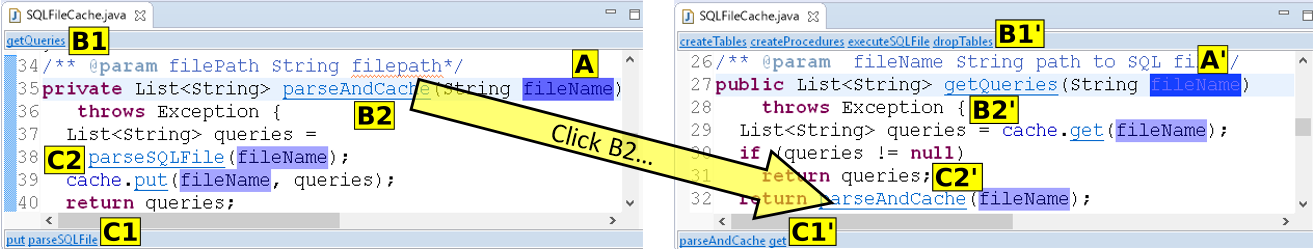
\includegraphics[width=\textwidth]{images/toolScreenshot}
	\caption{Code view in the Eclipse IDE with \textit{Flower} invoked during Task 1. The image on the left shows the tool running in the method \texttt{parseAndCache}. When the user clicks on the link in the editor (B1 or B2), they are taken to the function \texttt{getQueries}, which is a caller of \texttt{parseAndCache}.}	
	\label{fig:tool} 
\end{figure*}

\section{Flower}
\textit{Flower} was designed to realize all of the principles described in Section \ref{DesignPrinciples}. 
We implemented \textit{Flower} as a plugin to the Eclipse IDE~\cite{Eclipse}. 
We chose Eclipse because it is one of the most widely used open source IDEs for Java development and it provides many extension points for plugins. 
\textit{Flower} extends \emph{Call Hierarchy}, using its search functionality to track the flow of data across methods. 
Leveraging Eclipse's incremental compiler and JDT core, \textit{Flower} also implements several AST visitors to detect proper and up-to-date variable references.

When active, \textit{Flower} makes two modifications to Eclipse's user interface. 
First, it highlights on-screen references to selected variables.
Second, when references to the selected variable appear off-screen -- either elsewhere in the current method or in other methods -- \textit{Flower} adds links to those locations above and below the code view as well as to the code itself. 
Figure \ref{fig:tool} depicts \textit{Flower} invoked on a variable participants were asked to inspect as part of our evaluation. We also provide a 
video\footnote{Screen cast of \textit{Flower}: \url{https://figshare.com/s/39eadd74502a014ae018}} 
and virtual machine 
image\footnote{VM containing \textit{Flower}: \url{https://figshare.com/s/76aa260f21cf4233dc1c}}
demonstrating \textit{Flower} online.
To visualize how a programmer would interact with \textit{Flower}, consider the following scenario, which corresponds with Figure \ref{fig:tool}:
%	\url{tinyurl.com/FlowerDemo}} 

Suppose you are a programmer and you notice that by tampering with the value of the \texttt{fileName} variable, malicious users could gain access to sensitive information in the database. 
You want to determine whether users can modify \texttt{fileName} before it gets passed into \texttt{parseAndCache}. 
First, you click on \texttt{fileName} (A).
Much like \emph{Mark Occurrences}, \textit{Flower} is automatically invoked.
To help you locate where the variable is modified and referenced, \textit{Flower} highlights occurrences of that variable in the code.
Since \texttt{fileName} is a formal parameter to \texttt{parseAndCache}, any method calling \texttt{parseAndCache} could modify \texttt{fileName}. 
Those methods reside in other files, so \textit{Flower} provides links to their locations (B1).
Rather than move your mouse up to the top of the editor window, you click on \texttt{parseAndCache} (B2), which conveniently links to the first call site, \texttt{getQueries}. 
\textit{Flower} opens \texttt{getQueries} and highlights the location in that method where \texttt{fileName} passed to \texttt{parseAndCache} and shows that the value is passed to \texttt{getQueries} from \texttt{createTables}, \texttt{createProcedures}, \texttt{executeSQLFile}, and \texttt{dropTables} as seen in Fig. \ref{fig:tool}.  

%Something about using Flower for down flow.
%(A) - When a user clicks on a variable all (visible) instances of that variable are highlighted in the code. (B) - When the variable has been declared as a parameter to the current method, users can click on that method's name in the editor to navigate to a location where that method is called. (X) - When the variable is passed to an external method, users can click on that method's name to open its declaration. (C) - If the variable is passed in from another method or is defined earlier in the current file, a link to that location is displayed in the ``top box.'' (D) - If the variable is passed in to another method or referenced later in the current file, links to those locations appear in the ``bottom box.''


\section{Preliminary Evaluation}
We performed a preliminary evaluation of \textit{Flower} with eight programmers performing two code navigation tasks.\footnote{Study materials at: 
	%\url{tinyurl.com/flowerTool}}
	\url{https://figshare.com/s/49edec2b4810fbf5b2a0}}
As a baseline, we compare our tool against the existing suite of tools available in Eclipse (\emph{Open Declaration}, \emph{Mark Occurrences}, and \emph{Call Hierarchy}).
Our goals in this study were to (a) determine what types of navigation activities \textit{Flower} effectively supports and fails to support and (b) get feedback on the usability of \textit{Flower}.
To answer (a), we measured how quickly and accurately participants completed different activities.
The remainder of this section describes our participants, study design, and task selection, then concludes with our approach to answer (b).

All participants were graduate students at the time of the study with a mean of five years of professional programming experience. 
We recruited participants using a convenience sampling approach. 

Each participant used \textit{Flower} for one task and Eclipse's tools for the other task.
To control for learning and fatigue effects, we permuted the order participants received each tool and performed each task. 
Before the study, we asked participants to report whether they were familiar with the Eclipse IDE. This information helped us balance Eclipse novices across groups.

We based our tasks in this study on two tasks (Tasks 1 and 3) from a prior study~\cite{Smith2015}.
For these tasks, participants navigated across several classes in an open source Java medical records application containing over 50,000 lines of code.
In the previous study, participants used a think-aloud protocol to, among other things, describe their program navigation strategies.
Here, we did not interrupt, prompt, or ask participants to think aloud until after they had completed the tasks, as to not distort their task completion time.

The two tasks we chose are complementary in that Task 1 required participants to navigate up the call graph, inspecting the callers of the initial method. 
On the other hand, Task 2 required participants to inspect the methods called by the initial method.
For Task 1, we asked participants to tell us whether a method ever receives user-provided input.
For Task 2, we asked participants to tell us whether a form field is validated before being sent to the database.
To ensure all participants had a baseline familiarity, we trained participants on the appropriate tools preceding each task. 
To evaluate the effectiveness of the navigation tools rather than participants' familiarity with a particular code base, we asked participants to navigate code they had not previously contributed to. 

%We chose two tasks that (differentiate between the two tasks... up and down?)
We collected screen and audio recordings of each participant's tasks.
To evaluate the usability of \textit{Flower}, we administered an adapted version of the Post-Study System Usability Questionnaire (PSSUQ)~\cite{Lewis95ibmcomputer}. We modified the questionnaire by replacing ``this system'' with ``this tool'' and asked questions from the System Quality and Interface Quality categories.
To prompt discussion about the usability of \textit{Flower}, we also asked participants open-ended questions based on applicable categories from Nielsen's usability heuristics~\cite{Nielsen1992}.
%To capture participant's experiences that these two metrics overlooked, two of the authors independently examined each audio/video recording and recorded memos. 


\section{Results}
Here we present the results of our preliminary evaluation. 
We tested whether participants performed differently --- in terms of task completion time and correctness --- using the full suite of Eclipse tools, compared with Flower. 
We tested overall task completion time using two-tailed, unpaired, two-sample, t-tests and task correctness using chi-squared tests. 
The tests failed to identify a significant difference in completion time and correctness between \textit{Flower} and the Eclipse suite of tools. 
In the remainder of this section, we present our observations about the types of activities \textit{Flower} seemed to support.
We organize these results thematically into three topics:

%\begin{figure}
%	\centering
%	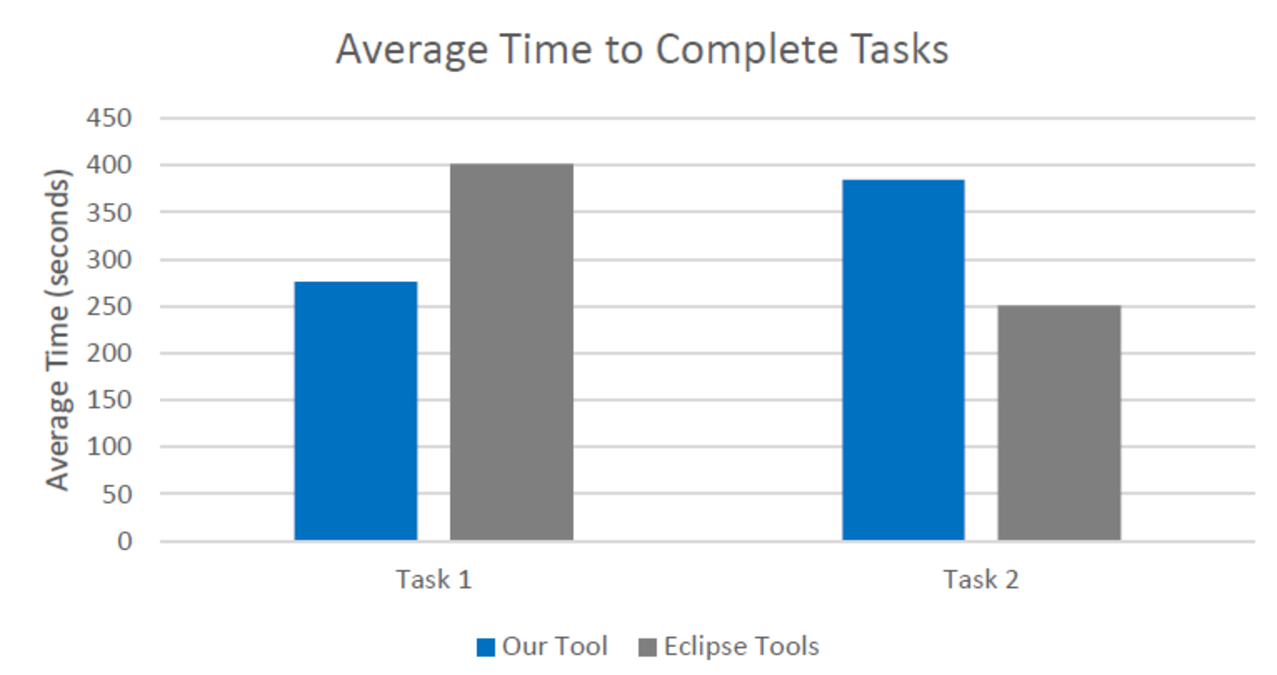
\includegraphics[width=\columnwidth]{images/taskTime}
%	\caption{Mean time to complete each task with and without Flower}
%	\label{fig:taskTime} 
%\end{figure}

\textbf{Approachable Interface:}
Compared to other PSSUQ questions, participants responded most positively to the three questions about \textit{Flower's} simplicity, how easy it was to use, and how easy it was to learn. 
These responses seem to indicate that participants were most enthusiastic about \textit{Flower's} minimalistic interface. 
Participants reiterated these sentiments in their responses to the open-ended questions. 
For the most part, participants felt it was easy to remember how to use \textit{Flower} and that it featured a ``consistent interface.''

\textbf{Branchless Navigation:}
For Task 1, all participants correctly navigated up the call graph and did so faster with \textit{Flower} compared to the Eclipse tools.
With \textit{Flower}, participants' mean completion time was 276 seconds, compared to 402 seconds with the Eclipse tools.

The first two steps in this task involved navigating a portion of the call graph that did not include any branches.
In other words, participants started in the \texttt{parseSQLFile} method, which was only called in one location, \texttt{parseAndCache}. 
The \texttt{parseAndCache} method was only called in one method \texttt{getQueries}.
Participants equipped with our tool were strictly faster in navigating the first step up this branchless chain. 
The mean times for participants to reach \texttt{parseAndCache} with \textit{Flower} and the Eclipse tools were 8 seconds and 44 seconds, respectively.
These two results suggest that \textit{Flower} successfully adhered to the \textsc{Low Barriers to Invocation} design principle. 

\textbf{Branching and Backtracking:}
For Task 2, participants were more accurate with \textit{Flower}.
Two participants (P3 and P6) navigated to the correct validation method with \textit{Flower}.
Only one (P8) did so with the Eclipse tools.

However, the mean completion time for Task 2 with \textit{Flower} was higher (385 seconds) compared to the Eclipse tools (251 seconds).
Additionally, participants who used \textit{Flower} for Task 2 scored the tool lower on the PSSUQ than those who used it for Task 1.
Based on open-ended responses and our observations of participants, we provide one likely explanation for this deficiency.
Participants were required to sift through more variable references and method calls to complete Task 2.
In navigating this more complex program structure, when participants took missteps they found it difficult to backtrack.
%Broken example... P6 was dissatisfied with back buttons while using Eclipse tools
%While working on Task 2 with Flower P6 attempted to use Eclipse's built-in back buttons to backtrack, but still had difficulty reorienting himself. 
To a lesser extent, we observed this same difficulty during Task 1.
After navigating through several chains of method invocations with \textit{Flower}, P7 felt like she had reached a ``dead end'' and was unsure of how to navigate back to where she came from.
Similarly, after reaching a top-level method, P1 asked, ``How can I return back to where I came from?''

%PSSUQ responses support this. Could talk about the low categories
%On the other hand, participants responded most negatively to questions about whether the tool provided all the expected functions and capabilities and whether it would enable them to complete tasks quickly.
%All the functions I expected (Missing tracability and mark bars, ... )
%To these two questions, participants' median response was 5. 


%Overall, task competion time distorts the actual time participants took to complete the task.
%Participants who explored more of the call graph are penalized. 
%Some participants spent additional time exeploring after finding the right answer to confirm their conclusion

%(Not sure how to report correctness here... 4 gave the correct answer with eclipse tools --
%2 were correct with ours. However, the incorrect two navigated correctly, located a hard-coded %parameter, responded incorrectly, and did not justify)
%However, participants were Y\% slower for Task 2.
%(Correctness in terms of navigation was even split. One with our tool guessed correctly)

%To understand why participants were faster for Task 1 with Flower, we analyzed how long it took participants to navigate one step up the call graph. 

%DFS exploration stategies

%\begin{table}
%	\centering
%	\caption{Participant Demographics}
%	\begin{tabular}{cSScc}
%		\rowcolor{Gray}
%		\hline
%		\multicolumn{1}{c}{\textbf{Participants}} & \multicolumn{1}{c}{\textbf{Industry}} & \multicolumn{1}{c}{\textbf{Java}} &\multicolumn{1}{c}{\textbf{Eclipse}} & \multicolumn{1}{c}{\textbf{Task}} \\
%		\rowcolor{Gray}
%		\multicolumn{1}{c}{ } & \multicolumn{1}{c}{\textbf{Exp.} \textit{(years)}} & \multicolumn{1}{c}{\textbf{Exp.} \textit{(years)}} & \multicolumn{1}{c}{\textbf{Exp.}} & \multicolumn{1}{c}{\textbf{Group}}\\
%		\hline
%		P1 & 9 & 5 & \checkmark & T1* - T2 \\
%		\rowcolor{Gray}
%		P2 & 0 & 6 & \checkmark & T2* - T1\\
%		P3 & 3 & 2 & - & T1 - T2*\\
%		\rowcolor{Gray}
%		P4 & 5 & 0 & - & T2 - T1*\\
%		P5 & 12 & 10 & \checkmark & T1* - T2\\
%		\rowcolor{Gray}
%		P6 & 0 & 3.5 & \checkmark & T2* - T1\\
%		P7 & 1 & 9 & \checkmark & T1 - T2*\\
%		\rowcolor{Gray}
%		P8 & 5.5 & 3.5 & \checkmark & T2 - T1*\\
%		\multicolumn{5}{c}{* Used Flower for task}
%	\end{tabular}
%	\label{table:participants}
%\end{table}

\section{Discussion}

\subsection{Systematic Navigation}
Participants completed simple navigation tasks quickly and accurately with \textit{Flower}, perhaps due to its minimalistic interface.
However, when the task required participants to navigate more complex semantic structures, participants demanded features that would allow them to navigate more systematically.
Many existing tools support systematic exploration through the use of secondary views containing either hierarchically structured lists of methods (e.g. \textit{Call Hierarchy} and \textit{Analyze Data Flow}) or call graph visualizations (e.g. \textit{Reacher~\cite{Reacher}}).
In keeping with \textit{Flower's} minimalistic design and trying to preserve \textit{Flower's} \textsc{Low Barriers to Invocation}, we envision several design changes that might enable \textit{Flower}  to support more systematic navigation.
Similar to \emph{Whyline}~\cite{Whyline}, \textit{Flower}  could use animation to transition more smoothly between locations, perhaps giving users a sense of naturally moving through the code.
By tracking developers' progress, \textit{Flower} could also display already-visited locations differently than unexplored methods either positionally or using colors:

\noindent
\includegraphics[width=\columnwidth]{images/HyperlinkColoring}

 %Especially important when participants reach ``dead ends.'' When we detect that, intervene!
%animations, breadcrumbs, detect dead ends, reorganize links to 


\subsection{Synergistic Tools}
Navigation without tool support can be frustrating and unfruitful.
However, full-featured navigation tools might be too cumbersome for simple navigation tasks and too complex for unfamiliar users.
We envision \textit{Flower} serving as a stepping stone to more sophisticated navigation tools. 
The design principles of \textsc{Low Barriers to Invocation} and \textsc{In Situ Navigation} enable users to quickly begin navigating using \textit{Flower}. 
We imagine that \textit{Flower} could detect when users reach ``dead ends'' or code that contains many complex branches.
Upon detecting one of these situations, \textit{Flower} could facilitate the user's transition to a more heavy-weight tool by either recommending or automatically invoking a tool that features additional navigation visualizations.
%For the purposes of this evaluation we observed programmers using Flower  in isolation.   

	
%Overwhelmed when the call graph had a high branching factor.
%	Participants quickly navigated up single paths as in Task 1
%	When call paths branched in many directions our tool could reccomend more full featured tools.\\


%Performance.
%Whenever the user clicks on a new variable Flower  has to search through the entire project for locations where the method is declared or invoked. We observed that participants navigated within one file more often than between files. To improve the performance of our tool, we could optimize the search to return local results before returning global search results.	Participants also repeated invocation on the same variables (we could do some caching)


\section{Study Limitations}
Our study had several limitations.
Due to the preliminary nature of this study, we recruited relatively few participants and only had them perform two tasks.
Although our study materials do not indicate we created \textit{Flower}, some participants may have deduced it was our tool.
As a result, participants may have inflated their positive responses to the PSSUQ due to social desirability bias.
Accordingly, we focus on participants' relative responses rather than their absolute values.
%Finally, we asked participants to navigate unfamiliar code.

\section{Conclusion}

In this work we presented a new tool, \textit{Flower}, that helps developers navigate program flow with its minimalistic interface. 
\textit{Flower} explores the void between tool-less navigation strategies and cumbersome flow visualization tools.
Based on our preliminary evaluation, \textit{Flower}  was most effective when developers wished to navigate program structures with few branches.

\section*{Acknowledgments}
We graciously thank our study participants for their time. 
We also thank Tyler Albert, Shubham Goyal, and members of the Developer Liberation Front for their thoughtful input. 
This material is based upon work supported by the National Science Foundation under grant number 1318323.



% trigger a \newpage just before the given reference
% number - used to balance the columns on the last page
% adjust value as needed - may need to be readjusted if
% the document is modified later
%\IEEEtriggeratref{8}
% The "triggered" command can be changed if desired:
%\IEEEtriggercmd{\enlargethispage{-5in}}

% references section

% can use a bibliography generated by BibTeX as a .bbl file
% BibTeX documentation can be easily obtained at:
% http://mirror.ctan.org/biblio/bibtex/contrib/doc/
% The IEEEtran BibTeX style support page is at:
% http://www.michaelshell.org/tex/ieeetran/bibtex/
\balance
\bibliographystyle{IEEEtran}
% argument is your BibTeX string definitions and bibliography database(s)
\bibliography{progNavPaper}


% that's all folks
\end{document}
